\documentclass[11pt]{beamer}
\usepackage[T1]{fontenc}
\usepackage[ngerman]{babel}
\beamertemplatenavigationsymbolsempty
\useoutertheme[subsection=false]{miniframes}
\setbeamertemplate{footline}[frame number]{}
\setbeamersize{text margin left=12.5mm,text margin right=10mm}


\usepackage{graphicx}

\usepackage{pgf, tikz}
\usetikzlibrary{shapes, automata, arrows, arrows.meta, positioning, decorations.pathreplacing, decorations.pathmorphing, calc, fit}
\usepackage{mathtools}

\usepackage[most]{tcolorbox}
\tcbuselibrary{xparse}
\usepackage{color}

\usepackage{multimedia}

%---------------------------------------------------------------
%colors

%base colors
\definecolor{wblau}{HTML}{B1D9EE}
\definecolor{blau}{HTML}{569BC0}
\definecolor{sblau}{HTML}{1E6B94}
\definecolor{worange}{HTML}{FFDFBA}
\definecolor{orange}{HTML}{FFBB6B}
\definecolor{sorange}{HTML}{E98F25}
\definecolor{gelb}{HTML}{c44848}

\definecolor{wgelb}{HTML}{F9E79F}

\definecolor{theorie}{HTML}{db6b94}
\definecolor{praxis}{HTML}{FFBB6B}
\definecolor{zukunft}{HTML}{569BC0}
%highlighting
\definecolor{wgruen}{HTML}{CAEA9C}
\definecolor{gruen}{HTML}{8FC542}
\definecolor{sgruen}{HTML}{2E4E00}
\definecolor{wviolett}{HTML}{D68FAF}
\definecolor{violett}{HTML}{B43C73}
\definecolor{sviolett}{HTML}{470021}

\definecolor{rot}{rgb}{.8,0,0}
\definecolor{rot2}{HTML}{E27D60}

\definecolor{turkis}{rgb}{0,.7,.7}

\definecolor{grau}{rgb}{0.47,0.47,0.47}
\definecolor{grau2}{rgb}{0.2,0.2,0.2}

\definecolor{titlebg}{HTML}{213845}
\definecolor{titlefg}{HTML}{F7E1C8}

%---------------------------------------------------------------------------

\usetheme{Singapore}
%	AnnArbor | Antibes | Bergen |
%	Berkeley | Berlin | Boadilla |
%	boxes | CambridgeUS | Copenhagen |
%	Darmstadt | default | Dresden |
%	Frankfurt | Goettingen |Hannover |
%	Ilmenau | JuanLesPins | Luebeck |
%	Madrid | Malmoe | Marburg |
%	Montpellier | PaloAlto | Pittsburgh |
%	Rochester | Singapore | Szeged |
%	Warsaw
\usecolortheme{beaver}
%	albatross | beaver | beetle |
%	crane | default | dolphin |
%	dove | fly | lily | orchid |
%	rose |seagull | seahorse |
%	sidebartab | structure |
%	whale | wolverine
%\usefonttheme{professionalfonts}
%	default | professionalfonts | serif |
%	structurebold | structureitalicserif |
%	structuresmallcapsserif
%\useinnertheme{rectangles}
%	circles | default | inmargin |
%	rectangles | rounded
%\useoutertheme{infolines}
%	default | infolines | miniframes |
%	shadow | sidebar | smoothbars |
%	smoothtree | split | tree
\makeatletter
\AtBeginDocument{%
  {
    \usebeamercolor{section in head/foot}
  }
  \pgfdeclareverticalshading{beamer@headfade}{\paperwidth}
  {%
    color(0cm)=(white);
    color(1.25cm)=(white)%
  }
  \setbeamercolor{section in head/foot}{bg=}
}
\addtoheadtemplate{\pgfuseshading{beamer@headfade}\vskip-1.25cm}{}
\makeatother

\makeatletter
\setbeamertemplate{frametitle}{
    \ifbeamercolorempty[bg]{frametitle}{}{\nointerlineskip}%
    \@tempdima=\textwidth%
    \advance\@tempdima by\beamer@leftmargin%
    \advance\@tempdima by\beamer@rightmargin%
    \vspace*{-13pt} %%%%%%%%%%%%% For example insert shift to right
    % \hspace*{-8.1pt} %%%%%%%%%%%%% For example insert shift to right
    \begin{beamercolorbox}[sep=.435cm,center,wd=\the\@tempdima]{frametitle}
        \usebeamerfont{frametitle}%
        \vbox{}\vskip-1ex%
        \if@tempswa\else\csname beamer@ftecenter\endcsname\fi%
        \strut\insertframetitle\strut\par%
        {%
            \ifx\insertframesubtitle\@empty%
            \else%
            {\usebeamerfont{framesubtitle}\usebeamercolor[fg]{framesubtitle}\insertframesubtitle\strut\par}%
            \fi
        }%
        \vskip-1ex%
        \if@tempswa\else\vskip-.3cm\fi% set inside beamercolorbox... evil here...
    \end{beamercolorbox}%
}
\makeatother
\setbeamercolor{frametitle}{fg=titlefg,bg=titlebg}
\setbeamercolor{title}{fg=titlefg,bg=titlebg}
%---------------------------------------------------------------------------
\pgfdeclarelayer{TransLayer}
\pgfsetlayers{TransLayer,main}

\tikzset{
  AutomatonState/.style = {
      inner sep = 0pt,
      line width = 4pt,
      draw = titlebg!75!white,
      minimum size = 20pt,
      initial text = {Start},
      initial where = left,
      accepting/.style = {
        accepting by arrow,
        accepting text = {Ende},
        accepting where = right,
    },
  },
  AutomatonEdge/.style={
      draw=titlebg,
      -{Stealth[inset=0pt, width=5pt, length=5pt]},
      >={Stealth[inset=0pt, width=5pt,length=5pt]},
      shorten >=0pt,
      shorten <=-.5pt,
      line width=2pt,
  },
  AutomatonLabel/.style={ text=black, scale=1.2},
  Automaton/.style = {
      node distance=22mm,
      on grid,
      >=Latex,
      initial text=,
      initial where=below left,
      every node/.style={AutomatonLabel},
      every state/.style = {AutomatonState},
      every edge/.style = {AutomatonEdge},
  },
  Box/.style = {
    line width = 1.5pt,
    rounded corners = 2pt,
  },
}
%---------------------------------------------------------------------------
\newcommand{\colorcircle}[1]{%
  \raisebox{0.25ex}{\tikz{\draw[line width=2pt, color=#1] (0,0) circle (2pt);}}%
}
\newcommand{\colorcross}[1]{%
  \raisebox{0.25ex}{\tikz{
    \draw[line width=2pt, color=#1] (-2pt,-2pt) -- (2pt,2pt);
    \draw[line width=2pt, color=#1] (-2pt,2pt) -- (2pt,-2pt);
  }}%
}
\newcommand{\yes}{\colorcircle{gruen}}
\newcommand{\no}{\colorcross{rot2}}

\newcommand{\gr}[1]{\textcolor{gruen}{#1}}
\newcommand{\vi}[1]{\textcolor{violett}{#1}}

\newcommand{\high}[3]{\only<-\number\numexpr#1-1\relax>{#3}\only<#1->{\textcolor{#2}{#3}}}
\newcommand{\shigh}[4]{\only<-\number\numexpr#1-1\relax,\number\numexpr#2+1\relax->{#4}\only<#1-#2>{\textcolor{#3}{#4}}}
\newcommand{\light}[2]{\shigh{#1}{#1}{gruen}{#2}}
 

%---------------------------------------------------------------------------
\title{Nutzen der Automatentheorie zur Verbesserung der Sicherheit durch Verifikation in IT-Systemen von KRITIS-Betreibern}
\author{Gustav Grabolle}
 \date{%
    Halle\\
    August 4, 2025
}
%---------------------------------------------------------------------------

\begin{document}

\maketitle

\begin{frame}
	\begin{tcolorbox}[ colframe=theorie, colback=theorie!35!white, height=2.3cm, valign = center, ]
		\huge
		\begin{center}
			Theoretische Grundlagen
		\end{center}
	\end{tcolorbox}

	\vfill

	\begin{tcolorbox}[ colframe=praxis, colback=praxis!35!white, height=2.3cm, valign = center, ]
		\huge
		\begin{center}
			Praktische Einsicht
		\end{center}
	\end{tcolorbox}


	\vfill

	\begin{tcolorbox}[ colframe=zukunft, colback=zukunft!35!white, height=2.3cm, valign = center, ]
		\huge
		\begin{center}
			KRITIS Einsatz
		\end{center}
	\end{tcolorbox}
\end{frame}

\setbeamercolor{background canvas}{bg=theorie!35!white}
\setbeamercolor{frametitle}{fg=theorie!35!white,bg=titlebg}

\begin{frame}{Was sind diese Automaten?}
	\visible<15->{
	\begin{minipage}{\textwidth}
		\begin{tcolorbox}[colframe=theorie, colback=white, valign=center, halign=center]
			\visible<15->{$\text{\light{15}{A}} \mathrel{\hat{=}} \text{Aufnahme}$} \hfill
			\visible<16->{$\text{\light{16}{B}} \mathrel{\hat{=}} \text{Bearbeitung}$} \hfill
			\visible<17->{$\text{\light{17}{E}} \mathrel{\hat{=}} \text{Einreichung}$}
		\end{tcolorbox}
		}
	\end{minipage}

	\vspace{10pt}

	\begin{minipage}{.48\textwidth}
		\begin{tcolorbox}[colframe=theorie, colback=white, valign=center, halign=center, height=170pt]
			\hspace*{-13pt}
			\begin{tikzpicture}[Automaton,]
				\node[state,initial, accepting] (q1) at (0,0) {};
				\node[state] (q2) [below of = q1] {};

				\draw[->] (q1) edge[bend left] node[AutomatonLabel, right]{\light{15}{A}} (q2);
				\draw[->] (q2) edge[loop below] node[AutomatonLabel, below] {\light{16}{B}} (q2);
				\draw[->] (q2) edge[bend left] node[AutomatonLabel, left]{\light{17}{E}} (q1);

				\only<3,6,9>{\draw[fill=gruen, draw=none] (q1) circle (7pt);}
				\only<4,5,10>{\draw[fill=gruen, draw=none] (q2) circle (7pt);}
				\only<11>{\draw[fill=rot2, draw=none] (q2) circle (7pt);}
				\only<4,10>{\draw[->] (q1) edge[bend left, draw = gruen] node[AutomatonLabel, right]{A} (q2);}
				\only<5>{\draw[->] (q2) edge[loop below, draw = gruen] node[AutomatonLabel, below] {B} (q2);}
				\only<6>{\draw[->] (q2) edge[bend left, draw = gruen] node[AutomatonLabel, left]{E} (q1);}
			\end{tikzpicture}
		\end{tcolorbox}
	\end{minipage}%
	\begin{minipage}{ .04\textwidth }%
		\hfill%
	\end{minipage}%
	\begin{minipage}{.48\textwidth}%
		\visible<2->{
			\begin{tcolorbox}[colframe=theorie, colback=white, valign=center, halign=center, height=60pt]
				\begin{tabular}{lc}
					\visible<2->{\light{4}{A}\light{5}{B}\light{6}{E}}  & \visible<7->{\yes}  \\
					\visible<8->{\light{10}{A}\shigh{11}{11}{rot2}{A}E} & \visible<12->{\no}  \\
					\visible<13->{ABEAE}                                & \visible<14->{\yes} \\
				\end{tabular}
			\end{tcolorbox}
		}
		\visible<19->{
			\begin{tcolorbox}[colframe=theorie, colback=white, height=103pt, valign=center, boxsep=0pt]
				\scriptsize
				\visible<19->{
					\textit{%
						Jede Aufnahme benötigt eine Einreichung, bevor eine neue Aufnahme erfolgt.
					}
				}
				\vfill
				\visible<20->{\[|u|_A = |u|_E \text{ oder } |u|_A = |u|_E + 1\]}
			\end{tcolorbox}
		}
	\end{minipage}
\end{frame}

\begin{frame}{Verifikation mit Modelchecking}
	\vfill
	\begin{center}
		\begin{tikzpicture}[
				node distance=0.5cm and 1.5cm,
				box/.style={
						draw=theorie,
						fill=white,
						line width = 1.5pt,
						rounded corners=3pt,
						minimum width=4cm,
						minimum height=0.8cm,
						align=center,
						inner sep=3pt,
						font=\normalsize,
					},
				arrow/.style={->, thick, draw=theorie}
			]


			% Linke Spalte
			\visible<1->{\node[box] (spec1) {\textbf{Spezifikation}};}
			\visible<2->{\node[box, below=of spec1] (spec2) {Logik};}
			\visible<4->{\node[box, below=of spec2] (spec3) {Automat $A_L$};}

			% Rechte Spalte
			\visible<1->{\node[box, right=of spec1] (real1) {\textbf{Realisation}};}
			\visible<2->{\node[box, below=of real1] (real2) {Programm};}
			\visible<5->{\node[box, below=of real2] (real3) {Automat $A_P$};}

			% Gleichheitszeichen zwischen spec1 und real1
			\visible<3->{\node at ($(spec1)!0.5!(real1)$) {\light{9}{\huge$\mathrel{\hat{=}}$}};}

			% Pfeile
			\visible<2->{\draw[arrow, AutomatonEdge] (spec1) -- (spec2);}
			\visible<4->{\draw[arrow, AutomatonEdge] (spec2) -- (spec3);}
			\visible<2->{\draw[arrow, AutomatonEdge] (real1) -- (real2);}
			\visible<5->{\draw[arrow, AutomatonEdge] (real2) -- (real3);}

			% Schnittfrage-Box
			\visible<6->{
				\node[fit=(spec3.east)(real3.west), inner sep=0pt] (fitbox) {};
				\path let \p1 = (real3.east),
				\p2 = (spec3.west),
				\n1 = {\x1 - \x2} in
				node[box, below=1.2cm of fitbox, minimum height=60pt, minimum width=\n1, text width=\n1-30pt] (check) {
						\only<7->{
							\scriptsize
							\textit{Gibt es einen erfolgreichen Lauf des Programmautomaten,\\ der kein erfolgreicher Lauf des Logikautomaten ist?}\\[10pt]
							\normalsize
							\only<-7>{
								\phantom{
									$L(A_P) \cap \overline{L(A_L)} = \emptyset$?
								}
							}
						}
						\only<8->{
							\normalsize
							$L(A_P) \cap \overline{L(A_L)} = \emptyset$\light{9}{?}
						}
					};
			}

			% Pfeile zur Schnittfrage
			\visible<6->{\draw[arrow, AutomatonEdge] (spec3.south) -- (check.north -| spec3.south);}
			\visible<6->{\draw[arrow, AutomatonEdge] (real3.south) -- (check.north -| real3.south);}
		\end{tikzpicture}
	\end{center}
	\vfill
\end{frame}

\setbeamercolor{background canvas}{bg=praxis!35!white}
\setbeamercolor{frametitle}{fg=praxis!35!white,bg=titlebg}

\begin{frame}{Modelchecking in Aktion: Promela+LTL+Spin}
	\begin{tcolorbox}[
			colframe = praxis,
			colback=white,
			valign=center,
			halign = center,
			left=-18pt,
			right=-18pt,
			top=0pt,
			bottom=0pt,
			boxsep=0pt,
			left skip = 20pt,
			right skip = 20pt,
			% sharp corners,
			arc = 0mm,
			boxrule = 4pt,
		]
		\movie[width=.877\textwidth]
		{
\includegraphics[width=.9\textwidth]{../sources/transparent.png}}{../sources/recording.mkv}
	\end{tcolorbox}

\end{frame}


\setbeamercolor{background canvas}{bg=zukunft!35!white}
\setbeamercolor{frametitle}{fg=zukunft!35!white,bg=titlebg}
\setbeamercolor{item}{fg=zukunft}

\begin{frame}{Modelchecking im Finanzwesen}
	\begin{minipage}[b][.7\textheight]{.5\textwidth}%
		\visible<2->{
			\begin{tcolorbox}[
					colframe = zukunft,
					left = 3pt,
					right = 3pt,
					right skip = 5pt,
				]%
				Model Checking and Verification of the Internet Payment System with \shigh{4}{7}{theorie}{SPIN}
				\footnotetext{
					\tiny
					Wei Zhang et al., Journal of Software, Vol. 7, No. 9, September 2012.
				}
			\end{tcolorbox}
			\vfill
			\begin{tcolorbox}[
					colframe = zukunft,
					left = 3pt,
					right = 3pt,
					right skip = 5pt,
				]
				\scriptsize
				Ergebnisse:
				\begin{itemize}
					\item<5-> Modell in Promela
					\item<6-> Spezifikation in LTL
					\item<7-> \gr{Erfolgreiche Verifikation des Modells}
				\end{itemize}
			\end{tcolorbox}
		}
	\end{minipage}%
	\begin{minipage}[b][.7\textheight]{.5\textwidth}
		\visible<3->{
			\begin{tcolorbox}[
					colframe = zukunft,
					skin=enhanced,
					interior style image = ./sources/massage-flow-format.png,
					height = 100 pt,
				]
				% 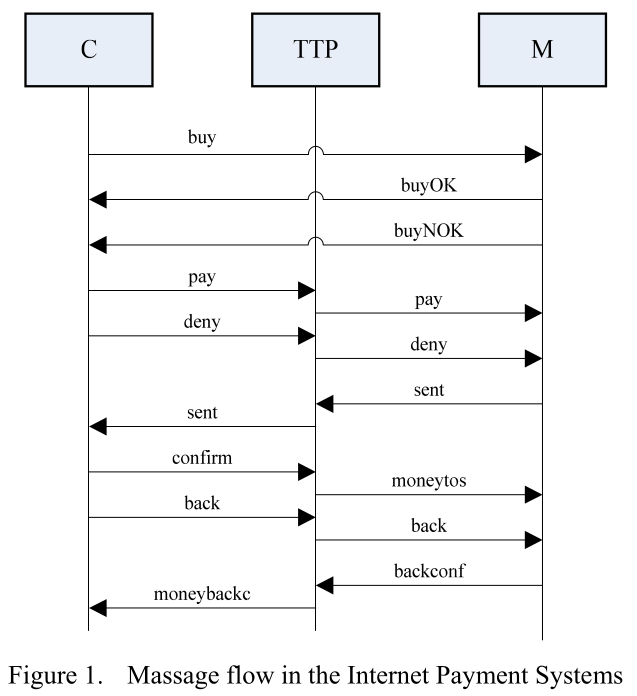
\includegraphics[height=90pt]{./sources/massage-flow.png}
			\end{tcolorbox}%
		}
		\vfill
		\visible<5->{
			\begin{tcolorbox}[
					colframe = zukunft,
					skin=enhanced,
					interior style image = ./sources/promela-channels.png,
					height = 60 pt,
				]
			\end{tcolorbox}
		}
	\end{minipage}
\end{frame}


\begin{frame}{Der Preis der Sicherheit}
	\vfill
	\begin{center}
		\begin{tikzpicture}[
				every node/.style = {
						draw = zukunft!50!white,
						line width =1.5pt,
						fill = white,
						inner sep = 0pt,
					}
			]
			\def\innerheight{35pt}
			\def\innerwidth{90pt}
			\def\sep{3pt}
			\visible<2->{
				\node[
					rounded rectangle,
					minimum height = \innerheight+2*\sep,
					minimum width=3*\innerwidth+4*\sep,
					draw = zukunft,
				] (p) at (0,0) {};
			}
			\visible<4->{
				\node[
					rounded rectangle,
					rounded rectangle right arc = none,
					minimum height = \innerheight,
					minimum width=\innerwidth
				] (p1) at ($(p)-(\innerwidth+\sep,0)$) {Programm 1};
			}
			\visible<5->{
				\node[
					rounded rectangle,
					rounded rectangle left arc = none,
					rounded rectangle right arc = none,
					minimum height = \innerheight,
					minimum width=\innerwidth
				] (p2) at (p) {Programm 2};
			}
			\visible<6->{
				\node[
					rounded rectangle,
					rounded rectangle left arc = none,
					minimum height = \innerheight,
					minimum width=\innerwidth
				] (p3) at ($(p)+(\innerwidth+\sep,0)$) {Programm 3};
			}
			\visible<3->{
				\node[
					rounded rectangle,
					minimum height = \innerheight+2*\sep,
					minimum width=3*\innerwidth+4*\sep,
					draw = theorie,
				] (v) at ($(p)-(0,2*\innerheight)$) {};
			}
			\visible<7->{
				\node[
					draw = theorie!50!white,
					rounded rectangle,
					rounded rectangle right arc = none,
					minimum height = \innerheight,
					minimum width=\innerwidth
				] (v1) at ($(v)-(\innerwidth+\sep,0)$) {Zertifikat 1};
			}
			\visible<8->{
				\node[
					draw = theorie!50!white,
					rounded rectangle,
					rounded rectangle left arc = none,
					rounded rectangle right arc = none,
					minimum height = \innerheight,
					minimum width=\innerwidth
				] (v2) at (v) {Zertifikat 2};
			}
			\visible<9->{
				\node[
					draw = theorie!50!white,
					rounded rectangle,
					rounded rectangle left arc = none,
					minimum height = \innerheight,
					minimum width=\innerwidth
				] (v3) at ($(v)+(\innerwidth+\sep,0)$) {Zertifikat 3};
			}

			\visible<2->{
				\node[draw = none, fill = none, text = zukunft!70!black] (pp) [above of = p] {\large \bf{Software}};
			}
			\visible<3->{
				\node[draw = none, fill = none, text = theorie!70!black] (vv) [below of = v] {\large \bf{Verifikation}};
			}

			\visible<7->{
				\path (p1.south) edge[AutomatonEdge] (v1.north);
			}
			\visible<8->{
				\path (p2.south) edge[AutomatonEdge] (v2.north);
			}
			\visible<9->{
				\path (p3.south) edge[AutomatonEdge] (v3.north);
			}
		\end{tikzpicture}
	\end{center}
	\vfill
	\visible<10->{
		\begin{tcolorbox}[
				colframe = zukunft,
			]
			Kosten Verifikation \hfill $
				\underset{\visible<11->{\text{\huge\vi{>}}}}{\overset{\visible<12->{\text{\huge\gr{<}}}}{\phantom{.}}}
			$ \hfill Kosten Systemausfall
		\end{tcolorbox}
	}
	\vfill
\end{frame}

\begin{frame}{Modelchecking in Bahnsteuerungssystemen}
	\begin{minipage}[b][.7\textheight]{.5\textwidth}%
		\visible<2->{
			\begin{tcolorbox}[
					colframe = zukunft,
					left = 3pt,
					right = 3pt,
					right skip = 5pt,
				]%
				Proving Completeness of Properties in Formal Verification of Counting Heads for Railways
				\footnotetext{
					\tiny
					Kinder, Sebastian, and Rolf Drechsler, 10th Euromicro Conference on Digital System Design Architectures, Methods and Tools (DSD 2007). IEEE, 2007.
				}
			\end{tcolorbox}
		}
		\vfill
		\visible<5->{
			\begin{tcolorbox}[
					colframe = zukunft,
					left = 3pt,
					right = 3pt,
					right skip = 5pt,
				]
				Verifikation in Minuten!
			\end{tcolorbox}
		}
	\end{minipage}%
	\begin{minipage}[b][.7\textheight]{.5\textwidth}
		\visible<3->{
			\begin{tcolorbox}[
					colframe = zukunft,
					skin=enhanced,
					interior style image = ./sources/ch-fm-model.png,
					height = 120 pt,
				]
				% 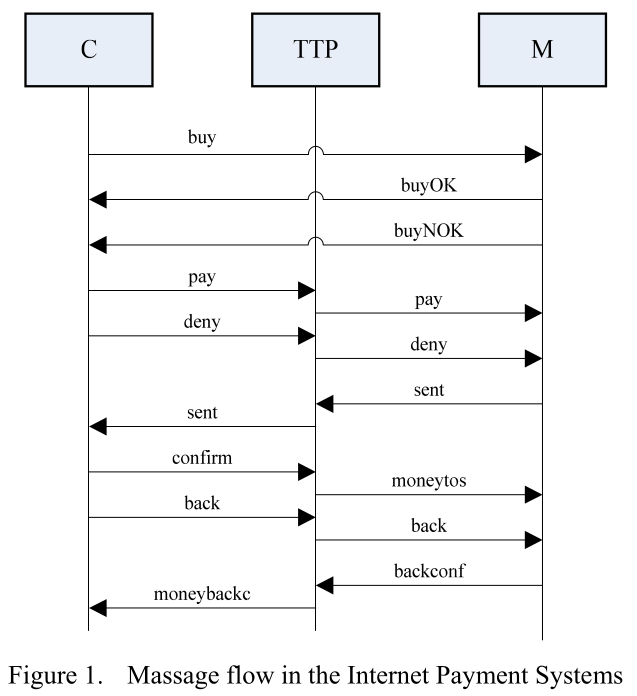
\includegraphics[height=90pt]{./sources/massage-flow.png}
			\end{tcolorbox}%
		}
		\vfill
		\visible<4->{
			\begin{tcolorbox}[
					colframe = zukunft,
					skin=enhanced,
					interior style image = ./sources/full-model.png,
					height = 40 pt,
				]
			\end{tcolorbox}
		}
	\end{minipage}
\end{frame}

\begin{frame}{Who will check the checkmen?}
	\visible<2->{
		\begin{tcolorbox}
			[
				colframe = zukunft,
				left = -2pt,
				right = 0pt,
			]%
			\vspace*{-10pt}
			\begin{align*}%
				 & \Box (
				\text{notfall} \rightarrow
				\Diamond \left(
					\text{alarm} \land
					\Box \left(
						\text{alarm} \rightarrow
						\bigcirc ( \text{alarm} \ \mathcal{U} \ \text{quittierung})
						\right)
				\right)                                                       \\
				 & \land\
				\Box \left(
					\text{quittierung} \rightarrow
					\mathcal{P} (\text{alarm})
				\right)                                                       \\
				 & \land\
				\Box \left(
					\text{alarm} \rightarrow
					\bigcirc (\neg \text{alarm} \ \mathcal{U} \ \text{quittierung})
				\right)                                                       \\
				 & \land\
				\Box \left(
					\text{quittierung} \rightarrow
					\bigcirc (\neg \text{alarm} \ \mathcal{U} \ \text{notfall})
				\right)                                                       \\
				 & \land\ \Diamond_{\leq 5} \left( \text{teamgerufen} \right) \\
				 & \land\
				\Box \left(
					\text{quittierung} \rightarrow
					\Diamond \left( \text{behebung} \land \text{grundzustand} \right)
				\right))                                                      \\
			\end{align*}
		\end{tcolorbox}
	}
	\begin{center}
		\visible<3->{
			\huge \textcolor{theorie}{Wo ist der Fehler?}
		}
	\end{center}
\end{frame}
\end{document}
